\chapter[Cơ sở lý thuyết và nghiên cứu liên quan]{Cơ sở lý thuyết và\\nghiên cứu liên quan}
\label{chap:background}

\section{MCI, dữ liệu dọc và bài toán tiên lượng}
Chương trước đặt ra bài toán xếp hạng nguy cơ tiến triển từ MCI. Để giải quyết bài toán đó, trước hết cần mô tả được sự khác nhau về diễn biến giữa người bệnh. MCI có thể ổn định, cải thiện hoặc tiến triển \cite{petersen2018mci}; các khung đánh giá bệnh Alzheimer cũng phân biệt biểu hiện nhận thức với bằng chứng bệnh lý từ dấu ấn sinh học \cite{jack2018niaaa}.

Dữ liệu dọc cho phép quan sát cả trạng thái tại từng lần khám lẫn sự thay đổi giữa các lần khám. ADNI cung cấp MRI và các đánh giá nhận thức, lâm sàng theo thời gian \cite{weiner2015impact}. Đây là cơ sở để mô hình học diễn biến thay vì chỉ dựa vào một ảnh chụp.

\section{Phân tích sống còn và mô hình thời gian}
\subsection{Biến cố, kiểm duyệt và Cox}
Do thời gian theo dõi mỗi người khác nhau, phân tích sống còn nghiên cứu thời gian đến biến cố; trong bài toán này, biến cố là đạt ngưỡng tiến triển nhận thức. Chẳng hạn, một người kết thúc theo dõi mà chưa có biến cố được ghi $\delta_i=0$: ta biết thời gian chưa tiến triển ít nhất dài bằng thời gian đã quan sát, nhưng chưa biết biến cố sẽ xảy ra khi nào. Mô hình Cox biểu diễn nguy cơ tức thời, với điều kiện chưa có biến cố trước $t$, bằng \cite{cox1972regression}
\begin{equation}
 h_i(t)=h_0(t)\exp(\eta_i).
\end{equation}
Mô hình gồm hai thành phần: điểm nguy cơ $\eta_i$ do mạng học được và hàm nguy cơ nền $h_0(t)$. Trong đó, $\eta_i$ cho biết người nào có xu hướng tiến triển sớm hơn, còn $h_0(t)$ mô tả nguy cơ tại từng thời điểm khi $\eta=0$. DeepSurv dùng mạng nơ-ron để học điểm nguy cơ phi tuyến trong cấu trúc Cox này \cite{katzman2018deepsurv}.

Tuy nhiên, điểm nguy cơ $\eta_i$ phản ánh nguy cơ tương đối giữa các cá thể, chưa cho biết xác suất tiến triển tuyệt đối tại một thời hạn cụ thể, chẳng hạn sau 3 năm. Muốn tính xác suất đó, cần ước lượng thêm nguy cơ tích lũy nền $H_0(t)$ từ thời gian theo dõi, biến cố và điểm nguy cơ trên tập huấn luyện. Sau đó, cần kiểm tra độ hiệu chỉnh, tức xem xác suất dự đoán có phù hợp với tỷ lệ biến cố quan sát hay không.

Khi thời điểm biến cố không trùng nhau, đối của log-hợp lý riêng phần là
\begin{equation}
\mathcal L_{\rm Cox}=-\sum_{i:\delta_i=1}\left[\eta_i-\log\sum_{j\in\mathcal R(t_i)}\exp(\eta_j)\right],
\end{equation}
trong đó $\mathcal R(t_i)$ gồm người còn được theo dõi và chưa có biến cố trước $t_i$. Breslow xử lý biến cố trùng thời gian \cite{breslow1974covariance}; C-index đánh giá thứ tự nguy cơ trên các cặp so sánh được \cite{harrell1996multivariable}.

Bên cạnh mô hình nguy cơ, phân tích sống còn cần một mốc bắt đầu theo dõi rõ ràng. Phương pháp dự đoán tại mốc xác định (landmarking) chọn người đủ điều kiện tại một thời điểm, rồi theo dõi biến cố từ thời điểm đó \cite{vanhouwelingen2007dynamic}. Mục~\ref{sec:study-design} trình bày hai mốc được dùng trong bộ dữ liệu của khóa luận.


\begin{figure}[H]
\centering
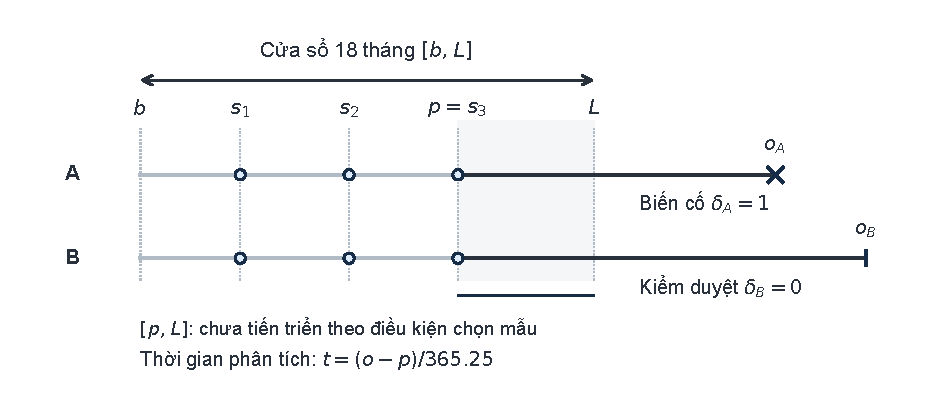
\includegraphics[width=\textwidth]{image/concept-survival.pdf}
\caption[Biến cố và kiểm duyệt phải]{Minh họa biến cố và kiểm duyệt: dấu nhân chỉ biến cố; vạch đứng chỉ thời điểm kết thúc theo dõi khi chưa ghi nhận biến cố.}
\label{fig:concept-survival}
\end{figure}

\subsection{T-LSTM và attention}
Để đưa lịch sử khám vào mô hình sống còn, LSTM tổng hợp chuỗi qua trạng thái ẩn, bộ nhớ và các cổng điều tiết \cite{hochreiter1997lstm}. Do khoảng cách giữa các lần khám không đều, T-LSTM bổ sung khoảng thời gian này vào phép điều chỉnh bộ nhớ \cite{baytas2017patient}. Sau đó, additive attention kết hợp các trạng thái bằng trọng số học được \cite{bahdanau2015attention}:
\begin{equation}
 e_t=\bm v^\top\tanh(W_hh_t+b_h),\quad
 \alpha_t=\frac{\exp(e_t)}{\sum_k\exp(e_k)},\quad z=\sum_t\alpha_th_t.
\end{equation}
Ở đây, $\alpha_t$ là trọng số mà mạng gán cho trạng thái tại lần khám $t$ khi tạo biểu diễn chung. Cấu hình T-LSTM và cách xử lý thời gian của mô hình cuối được trình bày ở Chương~\ref{chap:method}.

Có thể đọc Hình~\ref{fig:concept-longitudinal} theo hai bước: T-LSTM cập nhật thông tin từ các lần khám trước và xét khoảng cách thời gian; attention xác định mức đóng góp của từng trạng thái ẩn vào biểu diễn chung.

\begin{figure}[H]
\centering
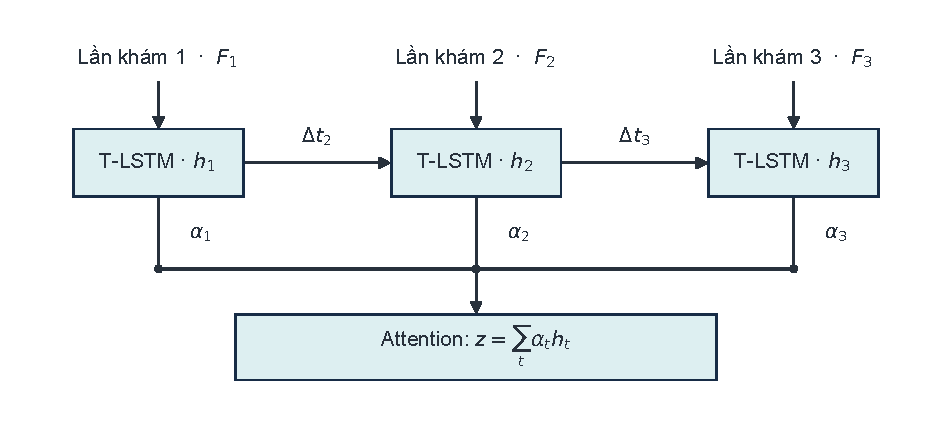
\includegraphics[width=\textwidth]{image/concept-longitudinal.pdf}
\caption[Tổng hợp thông tin qua các lần khám]{Sơ đồ khái niệm về dữ liệu dọc: khoảng thời gian giữa các lần khám và trọng số attention có vai trò khác nhau. Chi tiết phép cập nhật T-LSTM nằm ở Chương 3.}
\label{fig:concept-longitudinal}
\end{figure}

\section{Ba nguồn thông tin và biểu diễn}
\begin{table}[H]
\centering\small
\caption[Ba nguồn thông tin trong bài toán]{Thông tin chính của ba nguồn dữ liệu.}
\label{tab:background-inputs}
\begin{tabularx}{\linewidth}{@{}L{2.4cm}Y Y@{}}
\toprule
\textbf{Nguồn} & \textbf{Thông tin chính} & \textbf{Điểm cần lưu ý} \\
\midrule
MRI cấu trúc & Hình thái não; CNN học biểu diễn không gian & Cần chuẩn hóa và kiểm tra khác biệt miền ảnh \\
Radiomics & Phép đo hình dạng, cường độ và kết cấu & Phụ thuộc vùng não, chuẩn hóa và rời rạc hóa; có thể trùng thông tin MRI \\
Lâm sàng & MMSE, CDR và khả năng sinh hoạt & Liên quan tiêu chí biến cố; cần phân biệt thời điểm đo đầu vào với kết cục \\
\bottomrule
\end{tabularx}
\end{table}

Với nguồn ảnh, CNN 3D học quan hệ giữa các voxel trong thể tích. ResNet dùng kết nối residual để học phần hiệu chỉnh trên đầu vào \cite{he2016deep}; Med3D/MedicalNet cung cấp trọng số tiền huấn luyện ảnh y tế 3D \cite{chen2019med3d}. Khóa luận dùng ResNet-18 3D khởi tạo từ MedicalNet làm bộ mã hóa MRI chung cho các đối chứng chính. Li và cộng sự cũng cho thấy biểu diễn MRI có thể hỗ trợ tiên lượng, nhưng dùng hồi hải mã tại một thời điểm và đánh giá trên ADNI/AIBL, khác chuỗi MRI toàn não ở đây \cite{li2019hippocampal}.

Khác với đặc trưng học trực tiếp từ ảnh, radiomics biến MRI thành các phép đo định trước \cite{vangriethuysen2017computational}. Vì nhiều đặc trưng tương quan, PCA tạo các tổ hợp tuyến tính theo hướng phương sai lớn để giảm chiều \cite{jolliffe2016pca}. Các tham số PCA được học trên tập huấn luyện theo phương sai của đặc trưng; giá trị tiên lượng của biểu diễn sau giảm chiều được đánh giá bằng mô hình sống còn.

Để bổ sung thông tin chức năng, MMSE và CDR phản ánh nhận thức và chức năng sinh hoạt \cite{folstein1975mmse,morris1993cdr}. Các số đo ở lần khám đầu vào khác vai trò với đánh giá sau $L$ dùng tạo nhãn. Khi dữ liệu thiếu, chỉ báo quan sát giúp phân biệt giá trị đo thật với giá trị được điền; các biến và chỉ báo cụ thể được mô tả ở Mục~\ref{sec:preprocessing}.


\begin{figure}[H]
\centering
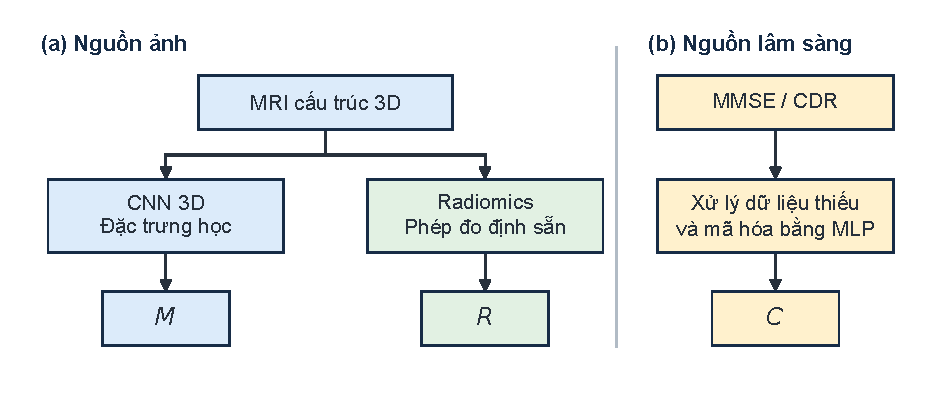
\includegraphics[width=\textwidth]{image/concept-sources.pdf}
\caption[Nguồn gốc của ba biểu diễn]{MRI và radiomics cùng xuất phát từ ảnh, nhưng cách tạo đặc trưng khác nhau. Dữ liệu lâm sàng bổ sung các đánh giá nhận thức và chức năng.}
\label{fig:concept-sources}
\end{figure}

\section{Hợp nhất thông tin và tham số hóa tương tác}
Để kết hợp các nguồn trên, mô hình cần đưa các biểu diễn về kích thước phù hợp \cite{baltrusaitis2019multimodal}. Có hai cách cơ bản: ghép nối giữ các vectơ cạnh nhau, còn tích ngoài tạo tường minh mọi tích chéo giữa hai vectơ \cite{zadeh2017tensor}. CP làm gọn trọng số dùng để xử lý các tích chéo này. Sau đó, cổng phần dư quyết định bổ sung bao nhiêu thông tin tương tác vào mỗi nguồn.


Hình~\ref{fig:concept-fusion} dùng hai vectơ hai chiều để phân biệt hai phép toán. Ghép nối chỉ xếp các tọa độ cạnh nhau; tích ngoài tạo thêm các tích giữa mọi cặp tọa độ. Lớp học sau đó mới chuyển những giá trị này thành đặc trưng phục vụ dự báo.

\begin{figure}[H]
\centering
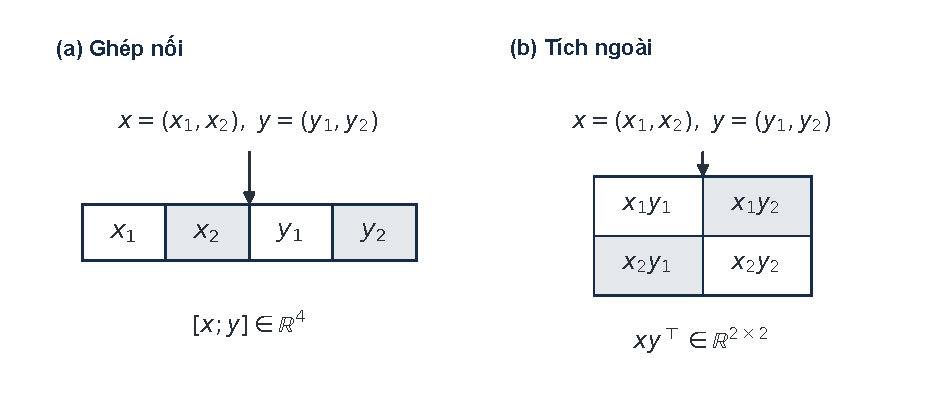
\includegraphics[width=\textwidth]{image/concept-fusion.pdf}
\caption[Ghép nối và tích ngoài qua ví dụ ký hiệu]{Ghép nối và tích ngoài của hai vectơ hai chiều.}
\label{fig:concept-fusion}
\end{figure}

\subsection{Từ tích ngoài đến CP}
Tích ngoài tạo các tương tác giữa mọi cặp đặc trưng của hai nguồn. Số tổ hợp tăng theo tích số chiều, khiến số trọng số cần học tăng nhanh. CP (CANDECOMP/PARAFAC, phân rã tensor thành tổng các thành phần hạng một) giúp thu gọn trọng số bằng các nhân tử hạng thấp. Hình~\ref{fig:cp-intro} minh họa hai cách tính; Chương~\ref{chap:method} trình bày ứng dụng cụ thể.
\begin{figure}[H]
\centering
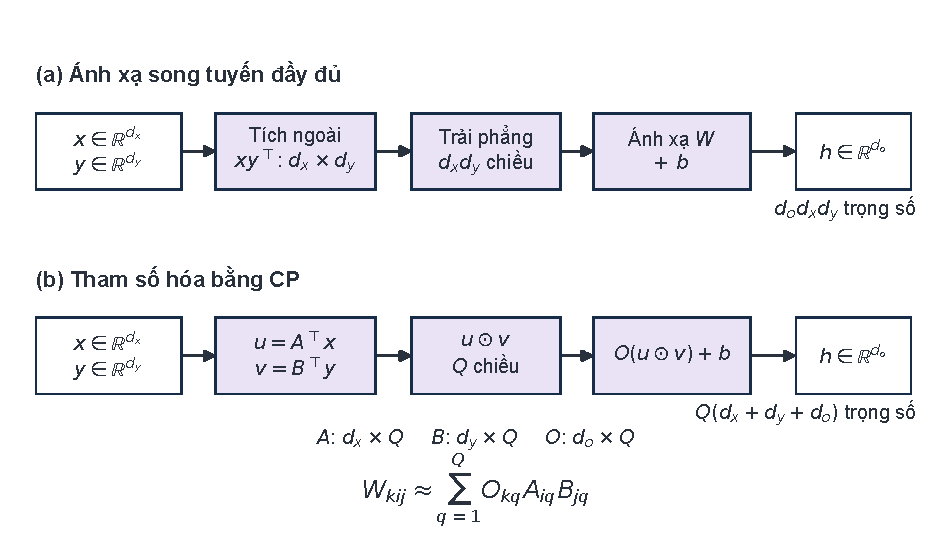
\includegraphics[width=\textwidth]{image/cp-concept-general.pdf}
\caption[Minh họa tích ngoài và CP]{Hai cách tính ánh xạ song tuyến với kích thước tổng quát: tích ngoài và tham số hóa CP hạng $Q$. Số trọng số trong hình chưa gồm hệ số chệch $b$.}
\label{fig:cp-intro}
\end{figure}
Với hai vector cột $x\in\mathbb R^{d_x\times1}$ và $y\in\mathbb R^{d_y\times1}$, tích ngoài $xy^\top\in\mathbb R^{d_x\times d_y}$ chứa mọi tích $x_iy_j$. Trải ma trận rồi áp dụng ánh xạ tuyến tính tương đương ánh xạ song tuyến:
\begin{equation}
 h_k=\sum_{i=1}^{d_x}\sum_{j=1}^{d_y}W_{kij}x_iy_j+b_k.
\end{equation}
Tensor trọng số $W\in\mathbb R^{d_o\times d_x\times d_y}$ có $d_od_xd_y$ phần tử. CP biểu diễn tensor bằng tổng các thành phần hạng một \cite{carroll1970candecomp,kolda2009tensor}:
\begin{equation}
 W_{kij}\approx\sum_{q=1}^Q O_{kq}A_{iq}B_{jq},\qquad
 h=O[(A^\top x)\odot(B^\top y)]+b.
\end{equation}
Số trọng số còn $Q(d_x+d_y+d_o)$, đổi lại giới hạn năng lực biểu diễn. Các nhân tử $A$, $B$ và $O$ được học trực tiếp trong mạng. Low-rank Multimodal Fusion (LMF, hợp nhất đa nguồn hạng thấp) dùng nhân tử hạng thấp cho hợp nhất \cite{liu2018lowrank}, còn Multimodal Tucker Fusion (MUTAN) dùng phân rã Tucker, trong đó tensor lõi kết hợp các nhân tử theo từng chiều \cite{benyounes2017mutan}; chúng cung cấp cơ sở cho việc khảo sát tham số hóa tương tác trong khóa luận.

\subsection{Gated residual}
Sau khi tạo tương tác, mô hình cần quyết định đưa bao nhiêu thông tin đó trở lại từng nguồn. Kết nối phần dư giữ đường biểu diễn gốc và cộng một phần bổ sung; cổng học từ đầu vào điều tiết phần bổ sung theo từng mẫu. Hai nghiên cứu dưới đây cung cấp cơ sở cho cách tổ chức này.

\paragraph{Ryumina và cộng sự: lấy văn bản làm nguồn neo.}
Text Residual Fusion kết hợp văn bản, âm thanh, khuôn mặt và cảnh để nhận dạng sự lưỡng lự \cite{ryumina2026residual}. Sau phép chiếu riêng, đặt $b=h_{\rm text}$ và $h_m$ là biểu diễn nguồn còn lại. Công thức (13) của bài báo có dạng
\begin{equation}
 g_m=\sigma(\operatorname{MLP}([b;h_m])),\qquad
 z=\operatorname{LN}\left(b+\sum_{m\ne\mathrm{text}}g_m d_m(h_m)\right).
 \label{eq:ryumina-residual}
\end{equation}
Ở đây, $[b;h_m]$ là ghép nối, $\sigma$ là sigmoid và $d_m$ là MLP tạo phần dư. Cổng xét đồng thời nguồn neo và nguồn bổ sung; tổng các phần dư được cộng vào văn bản rồi chuẩn hóa. Đặc trưng hợp nhất đi qua bộ phân loại. Hình~\ref{fig:literature-gates}(a) tóm tắt luồng này.

\paragraph{Liu và cộng sự: bổ sung chuyển động vào RGB.}
DyFADet+ dùng hai nhánh RGB và bộ xương, tạo các mức đặc trưng thời gian tương ứng để phát hiện cử chỉ \cite{liu2026motion}. Tại mức $\ell$, công thức (1)--(2) của bài báo là
\begin{align}
 G^{(\ell)}&=\sigma\left(\phi_\ell([F_r^{(\ell)};F_s^{(\ell)}])\right),\\
 F_f^{(\ell)}&=F_r^{(\ell)}+\alpha G^{(\ell)}\odot\psi_\ell(F_s^{(\ell)}).
 \label{eq:liu-residual}
\end{align}
$F_r$ và $F_s$ lần lượt biểu diễn RGB và bộ xương; $\phi_\ell$ là tích chập thời gian $1\times1$, còn $\psi_\ell$ là bộ chuyển đổi hai lớp tích chập với GELU. Cổng chọn mức bổ sung theo phần tử, còn $\alpha=0.5$ điều chỉnh cường độ chung. Các đặc trưng hợp nhất được đưa tới đầu phát hiện theo thời gian, như Hình~\ref{fig:literature-gates}(b).

\begin{figure}[H]
\centering
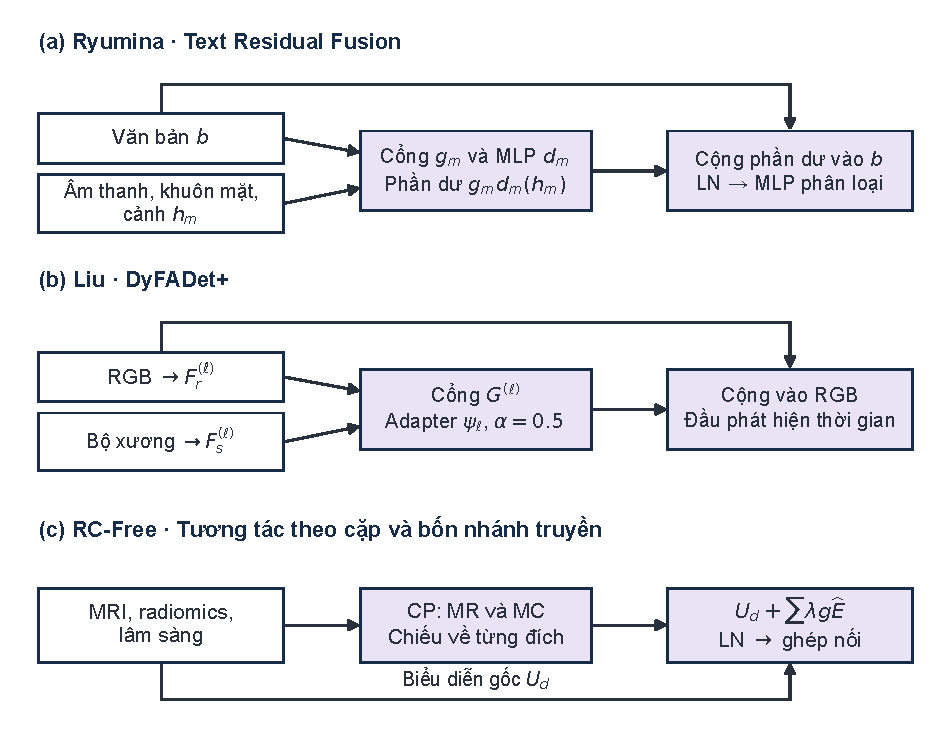
\includegraphics[width=\textwidth]{image/literature-gates.pdf}
\caption[Hai phương pháp phần dư có cổng và hướng thích nghi]{Sơ đồ khái quát được vẽ lại từ Ryumina và cộng sự \cite{ryumina2026residual} và Liu và cộng sự \cite{liu2026motion}. Các ô chỉ thể hiện luồng chính; dòng (c) là thiết kế của khóa luận.}
\label{fig:literature-gates}
\end{figure}

\paragraph{Từ hai ý tưởng trên đến thiết kế của khóa luận.}
Cơ sở thiết kế gồm ba bước. Thứ nhất, giữ biểu diễn gốc $U_d$ của từng nguồn để thông tin riêng vẫn có đường đi trực tiếp. Thứ hai, thay phần bổ sung từ một nguồn bằng đặc trưng tương tác CP của một cặp; phép chiếu riêng đưa tương tác về đúng số chiều của nguồn đích, tạo $\widehat E_{k\to d}$. Thứ ba, dùng cổng xét cả nguồn đích và phần bổ sung, rồi cộng các nhánh cùng đích:
\begin{equation}
 Z_d=\operatorname{LN}\left[U_d+\sum_{k\in\mathcal P(d)}\lambda_{k\to d}g_{k\to d}\widehat E_{k\to d}\right].
\end{equation}
Đây là lựa chọn kiến trúc dựa trên nguyên tắc phần dư có điều tiết. Trong RC-Free, MR (MRI--radiomics) truyền về MRI và radiomics; MC (MRI--lâm sàng) truyền về MRI và lâm sàng. Vì vậy, cả ba nguồn đều có đường gốc và bốn nhánh bổ sung được học riêng.

Hai hệ số đảm nhiệm hai vai trò khác nhau. $g_{k\to d}\in(0,1)$ là một số thay đổi theo người và lần khám, do MLP với sigmoid tạo ra. $\lambda_{k\to d}$ là tham số dùng chung của nhánh, khởi tạo bằng 0.1 và được học không ràng buộc dấu. Chẳng hạn, khi $\lambda=0.1$ và $g=0.2$, phần bổ sung trước phép cộng là $0.02\widehat E$; nếu $g=0.8$ thì thành $0.08\widehat E$. Như vậy, $\lambda$ đặt mức điều chỉnh chung, còn $g$ thay đổi mức tiếp nhận theo đầu vào. Khi $\lambda$ âm, hướng bổ sung đảo lại. LayerNorm chuẩn hóa tổng sau phép cộng; Mục~\ref{sec:gated-routing} trình bày đầy đủ phép chiếu và MLP của cổng.

\section{Nghiên cứu liên quan và hướng khảo sát}
\label{sec:related-work}
\begin{table}[H]
\centering\small
\caption[Tổng hợp nghiên cứu liên quan]{Các hướng nghiên cứu, phương pháp và thành phần được kế thừa.}
\label{tab:related}
\begin{tabularx}{\linewidth}{@{}L{3cm}Y Y@{}}
\toprule
\textbf{Hướng} & \textbf{Công trình và cách làm} & \textbf{Liên hệ với khóa luận} \\
\midrule
MRI đơn thời điểm & Li: biểu diễn hồi hải mã; Nakagawa: thể tích chất xám và mạng sống còn \cite{li2019hippocampal,nakagawa2020survival} & Cơ sở khảo sát biểu diễn ảnh và mục tiêu sống còn \\
Dữ liệu dọc & Li--Fan, Ding: nhận thức/MRI theo thời gian; Dong: học thay đổi từ cặp MRI \cite{li2019early,ding2023progression,dong2021deepatrophy} & Phân biệt học diễn biến với dự đoán biến cố tương lai \\
Radiomics và lâm sàng & Tang: LASSO--Cox, kết hợp thêm biến lâm sàng/xét nghiệm \cite{tang2021individualized} & Kiểm tra thông tin bổ sung trong cùng thiết lập \\
MRI dọc học sâu & Aghajanian: CNN--PCA--T-LSTM và attention \cite{aghajanian2025longitudinal} & Quy trình tham chiếu và cách đánh giá phân tầng nguy cơ \\
\bottomrule
\end{tabularx}
\end{table}

Trong các công trình ở Bảng~\ref{tab:related}, Aghajanian và cộng sự là tham chiếu gần nhất: 228 người MCI có ba MRI trong 18 tháng. CNN được huấn luyện trước, sau đó trích vector 512 chiều, dùng PCA giữ 99\% phương sai và đưa vào T-LSTM với attention \cite{aghajanian2025longitudinal}. Bài báo đánh giá điểm nguy cơ bằng C-index, KM và ROC tại các thời hạn. Radiomics chất xám chưa đem lại cải thiện nhất quán; mô hình cuối không giữ nguồn này. Kết quả này gợi mở việc khảo sát cách kết hợp biểu diễn ảnh với các nguồn bổ sung.

Từ quy trình này, bản \emph{Baseline Reproduction (CNN--PCA--T-LSTM)} của khóa luận kế thừa quy trình trên nhưng dùng 359 người, tiền xử lý và cấu hình khác. Đây là bản tái lập có điều chỉnh. RC-Free còn thay đổi cách hợp nhất và cấu hình huấn luyện, nên chênh lệch giữa hai quy trình không thể quy riêng cho CP hay cổng.

\subsection{Từ bằng chứng trước đến thiết kế nghiên cứu}
\label{sec:research-gaps}
Dữ liệu dọc có thể mô tả thay đổi, nhưng lợi ích tiên lượng cần được kiểm chứng thay vì mặc định tốt hơn ảnh đơn thời điểm. Tương tự, MRI và radiomics cùng nguồn ảnh nên có thể bổ sung hoặc lặp thông tin; biến lâm sàng còn liên quan trực tiếp tiêu chí kết cục. Vì vậy, các đối chứng đầu vào đóng vai trò thăm dò, còn trọng tâm là kiểm tra cách hợp nhất trong điều kiện so sánh rõ ràng.

Tương tác tường minh làm số tham số tăng theo tích số chiều. Khóa luận đối chiếu ghép nối với tích ngoài, rồi dùng CP để kiểm tra đánh đổi giữa kích thước lõi tương tác và C-index. Nghiên cứu cũng kiểm tra việc chỉ giữ MR (MRI--radiomics) và MC (MRI--lâm sàng). Kết quả nhiều lần khởi tạo và phân tích sống còn của RC-Free giúp mô tả khả năng phân biệt/phân tầng nguy cơ.

Như vậy, các nghiên cứu trước cung cấp từng thành phần nhưng chưa quyết định cách hợp nhất phù hợp cho nhóm dữ liệu hiện tại. Chương~\ref{chap:method} cụ thể hóa lựa chọn này thành quy trình dữ liệu, mô hình RC-Free và cách đánh giá.
